 %
\documentclass[11pt]{article}

\usepackage{times}
\usepackage{amsmath}
\usepackage{amsthm}
\usepackage{amssymb}
\usepackage{mathabx} 
\usepackage{graphicx}
\usepackage{color} 
\usepackage{setspace} 
\usepackage{rotating}
\usepackage{natbib}
\usepackage{multirow}
\usepackage{xspace}
\usepackage{lscape}
%\usepackage{cite}
\usepackage{xr}
\externaldocument{mcref}
\usepackage{bbm}


\usepackage{hyperref}
\urlstyle{rm}
\hypersetup{
  colorlinks,
  urlcolor=blue,
  linkcolor=black,Processor
  citecolor=black
}

% Text layout
\oddsidemargin 0in
\evensidemargin 0in
\topmargin -.5in
\textwidth 6.5in
\textheight 9in

\usepackage[labelfont=bf,labelsep=period,justification=raggedright]{caption}

% Remove brackets from numbering in List of References
\makeatletter
\renewcommand{\@biblabel}[1]{\quad#1.}
\newcommand{\smallCom}[1]{\marginpar{\tiny{#1}}}
\newcommand{\vect}[1]{\boldsymbol{\mathbf{#1}}}
\newcommand{\ld}{\mathcal{L}}
\newcommand{\ignore}[1]{}
\newcommand{\mcref}{\textsc{McRef}\xspace}
\newcommand{\E}{\mathbb{E}}
\newcommand{\X}{\vect{X}}
\newcommand{\M}{\mathcal{M}}
\newcommand{\Tr}{\mathcal{T}}
\newcommand{\B}{\vect{B}}
\newcommand{\Y}{\vect{Y}}
\newcommand{\G}{\vect{G}}
\newcommand{\T}{\vect{\Theta}}
\newcommand{\I}{\mathbb{I}}
\newcommand{\Ip}{\mathcal{I}(p,l)}
\newcommand{\Ib}{\mathcal{I}(b,l)}
\newcommand{\GT}{\G\T}
\newcommand{\Mref}{\M_{ref}}
\newcommand{\Mnull}{\M_{null}}
\newcommand{\Pref}{\widetilde{P}}
\newcommand{\rbf}{\text{BF}}
%\newcommand{\hbf}{\text{BF}}
\newcommand{\Om}{\Omega}
\newcommand{\GTref}{\widetilde{\GT}}
\newcommand{\Gref}{\widetilde{\G}}
\newcommand{\Tref}{\widetilde{\T}}
\newcommand{\1}{\mathbbm{1}}
\newcommand{\Z}{\vect{Z}}
\newcommand{\Zref}{\widetilde{\Z}}
\newcommand{\Omref}{\widet	ilde{\Om}}
\newcommand{\Fext}{F_{Z}}
\newcommand{\troot}{\theta_{root}}
\newcommand{\Gc}{\G_c}
\newcommand{\Gm}{\G_m}
\newcommand{\Mcomb}{\M_{\comb}}
\newcommand{\gp}{G-PhoCS }
\newcommand{\tmin}{\tau_{\text{min}}}

% Two lines from genres
\def\comb{\rotatebox[origin=c]{90}{$\exists$}}
\def\@cite#1#2{(#1\if@tempswa , #2\fi)}
\def\@biblabel#1{}

\usepackage[utf8]{inputenc}
\usepackage{amsmath}
\usepackage[normalem]{ulem}
\usepackage{color}
\usepackage{amsfonts}
\usepackage{listings}
\usepackage{amssymb}
\usepackage{amsmath}% http://ctan.org/pkg/amsmath
\usepackage[normalem]{ulem}
\usepackage{graphicx}
\usepackage[linesnumbered,lined,boxed,commentsnumbered,noend,ruled,vlined]{algorithm2e}




\usepackage[utf8]{inputenc}

% Default fixed font does not support bold face
\DeclareFixedFont{\ttb}{T1}{txtt}{bx}{n}{10} % for bold
\DeclareFixedFont{\ttm}{T1}{txtt}{m}{n}{10}  % for normal

% Custom colors
\usepackage{color}
\definecolor{deepblue}{rgb}{0,0,0.5}
\definecolor{deepred}{rgb}{0.6,0,0}
\definecolor{deepgreen}{rgb}{0,0.5,0}

\usepackage{listings}

% Python style for highlighting
\newcommand\pythonstyle{\lstset{
language=Python,
basicstyle=\ttm,
otherkeywords={self},             % Add keywords here
keywordstyle=\ttb\color{deepblue},
emph={recursive_num_coals,recursive_coal_stats},% Custom highlighting
emphstyle=\ttb\color{deepred},    % Custom highlighting style
stringstyle=\color{deepgreen},
frame=tb,                         % Any extra options here
showstringspaces=false            % 
}}


% Python environment
\lstnewenvironment{python}[1][]
{
\pythonstyle
\lstset{#1}
}
{}

% Python for external files
\newcommand\pythonexternal[2][]{{
\pythonstyle
\lstinputlisting[#1]{#2}}}

% Python for inline
\newcommand\pythoninline[1]{{\pythonstyle\lstinline!#1!}}



\graphicspath{ {images/} }
\author{Ron Visbord}
% \newcommand{\smallCom}[1]{\marginpar{\tiny{#1}}}
\title{Thesis!}

\begin{document}

\maketitle


\section{Calculations Schema}


\subsection{The Computational Objective}

Consider formula (\ref{eq:rbf}) for calculating the Bayes Factor of model $M$ relative to $\Mref$:
%
%
\begin{equation}
 \frac{1}{\rbf(\M:\Mref|\X)}  ~~\approx~~ \frac{1}{N} \sum_{i=1}^{N}\frac{\Pref(\GT^{(i)}|\Mref) }{P(\GT^{(i)}|\M)} ~ 
\end{equation}

Since the denominator $P(\GT^{(i)}|\M)$ is constantly calculated by \gp in the MCMC process, what remains for mcref to calculate in order to estimate the Bayes Factor is the model pairing conditional $\Pref(\GT^{(i)}|\Mref)$. This is composed of hidden variable likelihoods and the genealogy likelihood over the reference model. See equations $(\ref{eq:pref_null})$, $(\ref{eq:pref_mig})$ and $(\ref{eq:rbf_comb_nomig})$ for examples of realizations of this formula for different reference models. The following chapter addresses calculation of the \textbf{genealogy likelihood} efficiently, as it is the main component making up the model pairing conditional and represents the bulk of our computational challenge.\\

Killer connecting sentence.\\

We imagine the process of constructing a reference model as a series of transformations on the hypothesis model:
\begin{enumerate}
\item We First "collapse" some subtree of the hypothesis. 

Collapsing is the process of merging the populations of a subtree. "Clade-Collapsing" is the act of the merging all the populations of a subtree rooted at some population $P$ into a single population. This new population contains the portion of the genealogies previously located inside the subtree. We denote the resulting merged population $clade(P)$. Figure $(\ref{fig:clade_collapse_AB})$ illustrates a clade-collapsing of a subtree rooted at $AB$ into a new population, $clade(AB)$. 

Similiarly, "Comb-Collapsing" is the act of the merging populations of a subtree, while perserving its leaves up to the comb-age. 
See figure (\ref{fig:comb_collapse_and_split_interval}) for examples. We will formally describe this operation later.


\item We then map the hidden parameters of the hypothesis model onto parameters of the reference model s.t. the two conditions of a valid model-pairing function are met.
\end{enumerate}

Under this process, any part of the topology which is not transformed are mapped identically into the reference model. See for example populations $ABC$ and $C$ in figure \ref{fig:clade_collapse_AB}. This allows us, when calculating genealogy likelihoods, to reuse statistics gathered by \gp.

\begin{figure}[h]
\centering
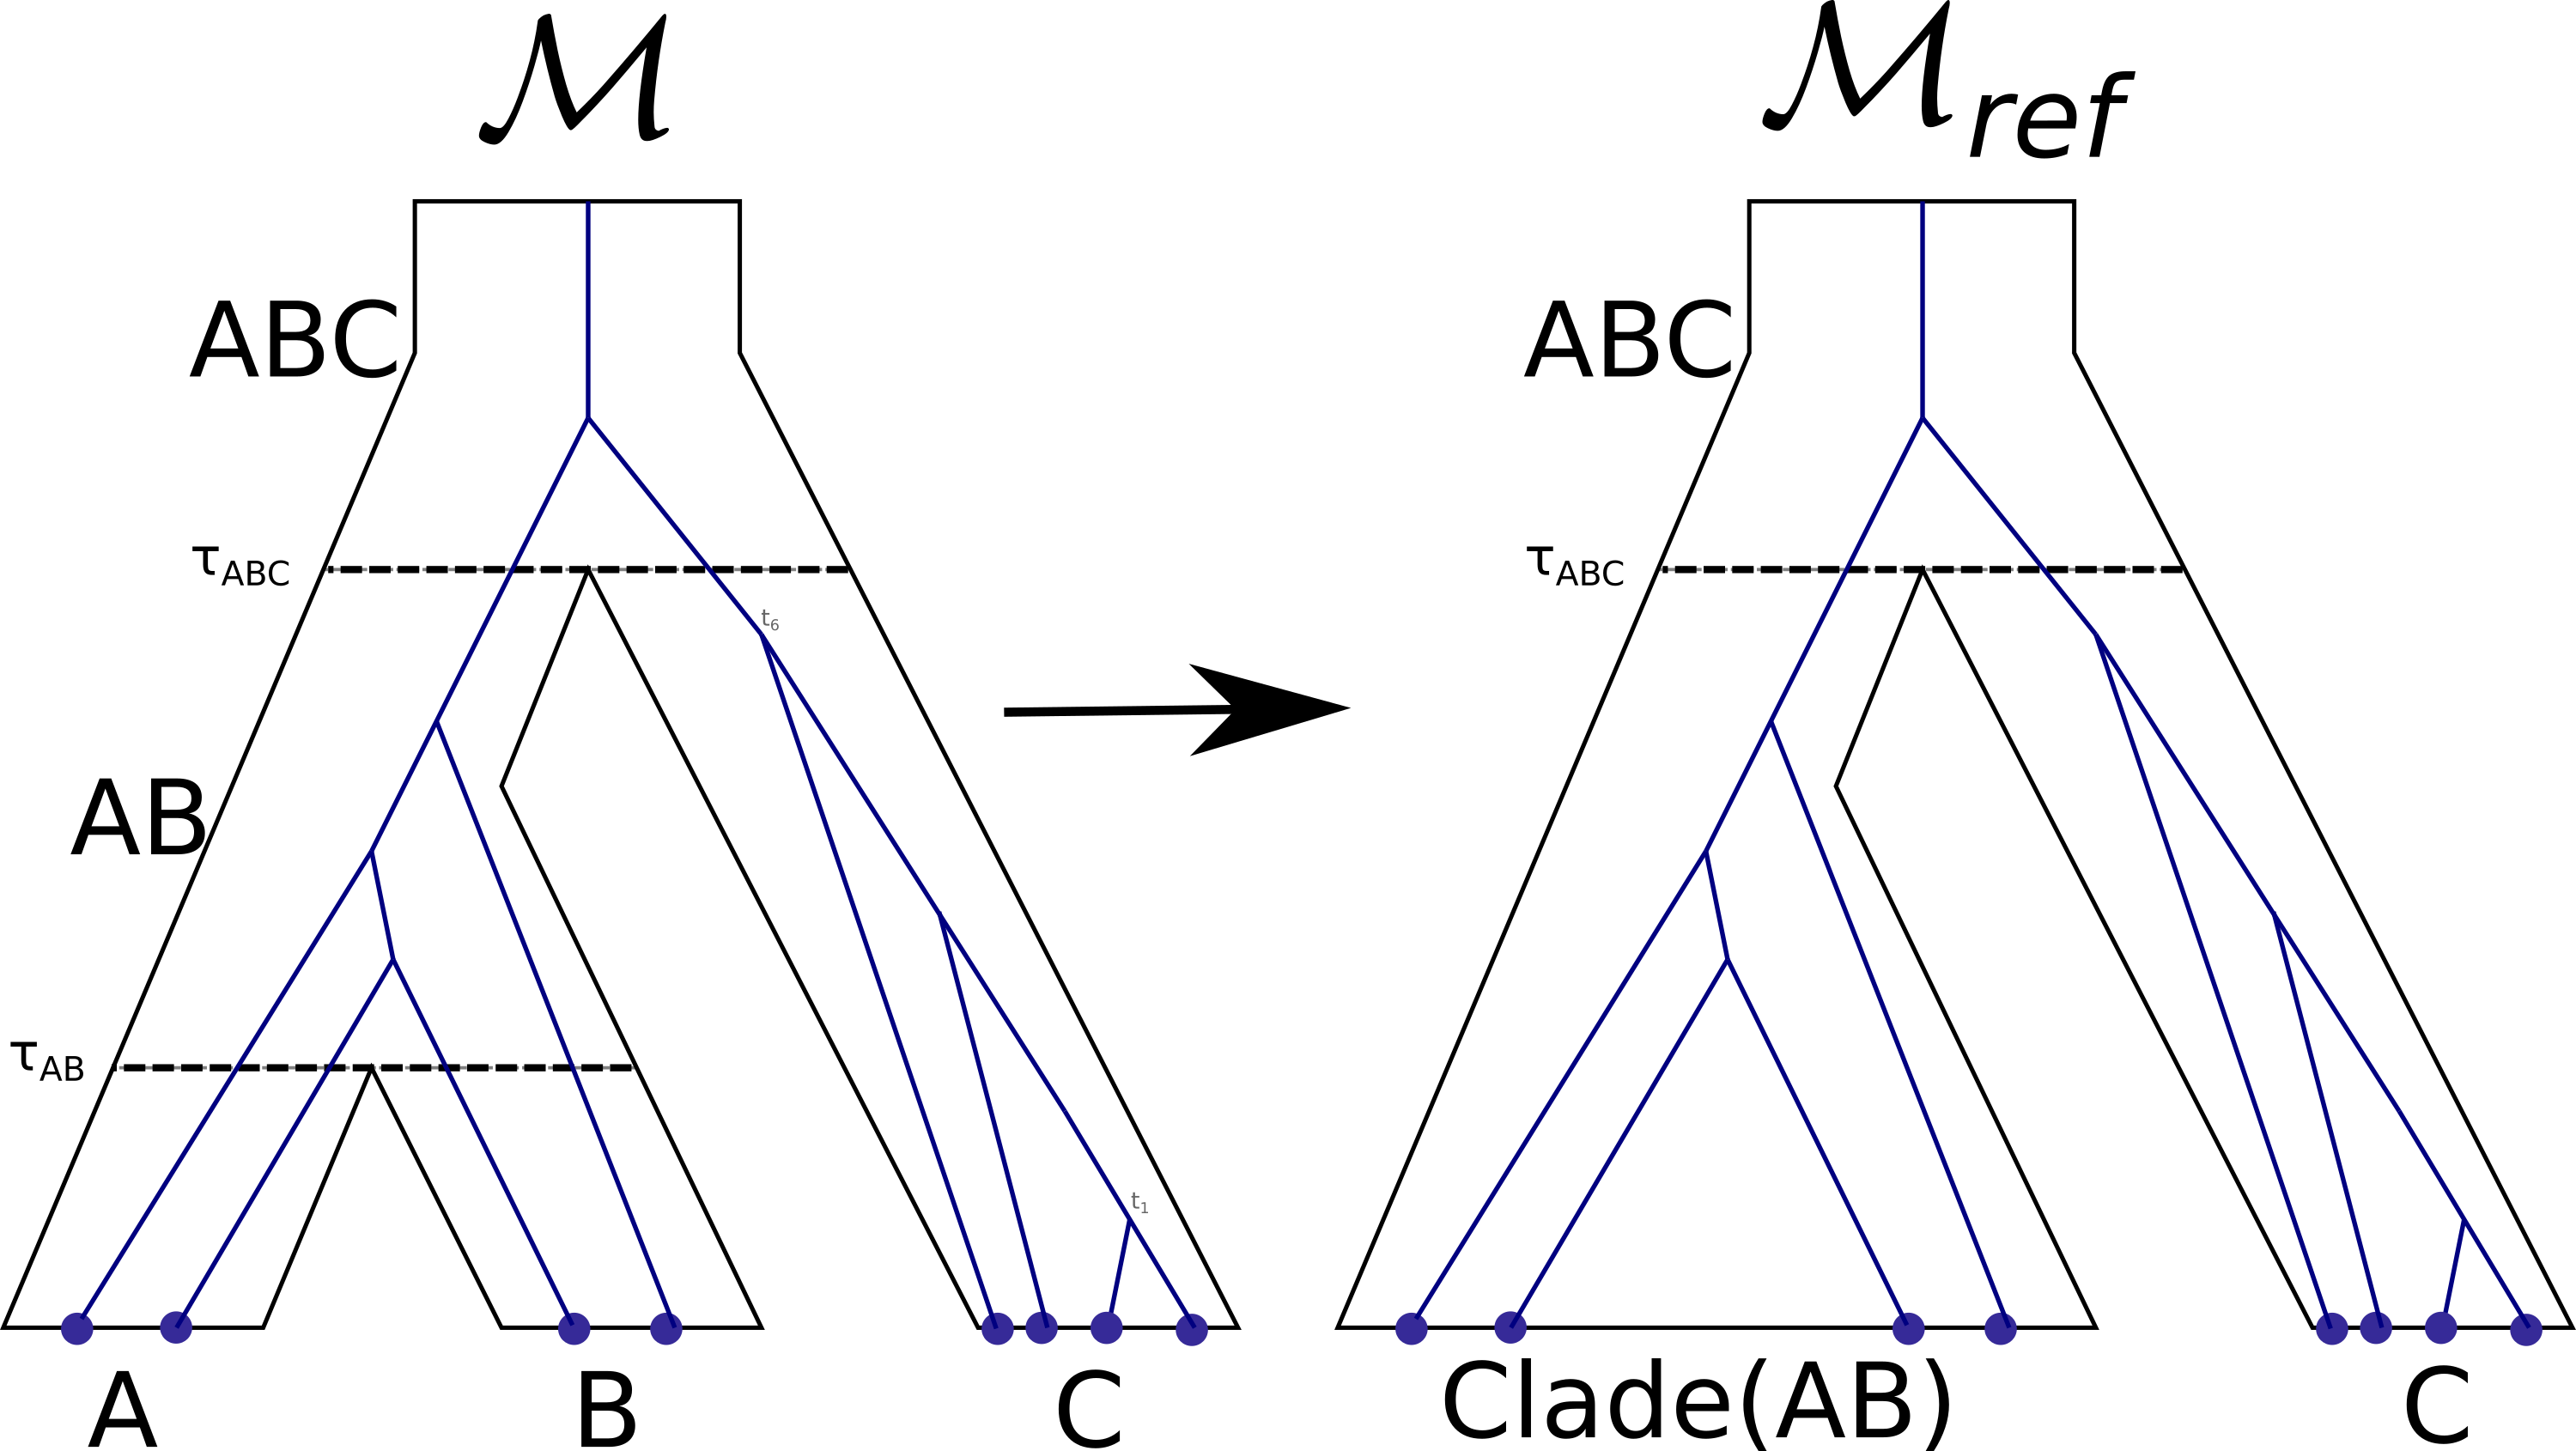
\includegraphics[width=0.8\textwidth]
{clade_collapse_AB}
\caption{\textbf{Construction of a reference model via clade-collapse - } The reference model  $\Mref$ is created by clade-collapsing population $AB$ and identically mapping the rest of the hypothesis. When calculating genealogy likelihood over the reference model, we reuse statistics  calculated by \gp for $ABC$ and $C$, and need only recalculate genealogy likelihood inside $clade(AB)$. This saves valuable effort in calculation of $P(\G|\T,\Mref)$ \textcolor{red}{TODO - Color-code the populations s.t. the reused stats are emphasized (Maybe fadeout the reused pops?). Also, move the arrow exactly in between the hypotheses}}
\label{fig:clade_collapse_AB}
\end{figure}


We note that there exists a natural trade-off between the flexibility in choice of reference model and the amount of data the MCMC process is required to emit. For example, if no flexibility is required and the reference model is predetermined before MCMC execution, formula (9) can be calculated during MCMC iteration and only the final RBF value need be emitted. However, calculating (9) on any other reference model would require another full run of MCMC.
%
On the other hand, the RBF for every reference model can be computed in post-processing if the MCMC prints out the full hidden state $\GT$ in each iteration.
%
However this would yield an unreasonable amount of traced information, in proportion to the size of the model and to the number of loci.


We designed a computational scheme that aims to find a reasonable middle ground between these two extreme options.
Our objective was to maximize the number of reference models we could consider after running a single MCMC sampling chain without blowing up the output trace.
This is done by identifying a collection of sufficient statistics for $\G$ that satisfy two conditions:
%
%
\begin{enumerate}
 \item The number of sufficient statistics depends on the complexity of the target model, $\M$, but not on the size of the data (i.e. the number of individuals and the number of loci).
 \item The sufficient statistics allow calculation of $P(\G|\T,\Mref)$ for a wide variety of reference models and values of model parameters (namely, migration rates and population sizes).
\end{enumerate}
%
%
\subsection{Efficient Sufficient Statistics for the Genealogy Likelihood $\mathbf{P(G|\Theta, \M)}$}

Sufficient statistics that satisfy these conditions are derived from the expression for the genealogy likelihood $P(\G|\T, \M)$ under Kingman's coalescent, which we briefly recall here.
First, because the loci are assumed to be freely recombining, then the local genealogies $\G=(G_1,...G_L)$ are conditionally independent given the model parameters and the likelihood may be expressed as a product of locus-specific likelihoods, $P(G_l|\T,\M)$ \textit{\# maybe put illustration of multiple loci?\#}.  Each locus-specific likelihood is a product of exponentially distributed waiting times for coalescent and migration events. The rates of these exponential distributions depend on the model parameters (population sizes and migration rates) as well as the number of lineages considered for coalescence and migration. We thus identify for each population the set of coalescent and migration events that change the number of lineages modeled in that population in $G_l$. Each time interval $I$ between two consecutive events is associated with the following properties:
\begin{itemize}
 \item $t(I)$ -- the elapsed time of the interval.
 \item $n(I)$ -- the number of lineages of $\G_l$ alive during that time in the target population.
 \item $isCoal(I)$ ~,~ $isInMig(I)$  -- binary values that indicate whether the event above the interval is a coalescent event or incoming migration event (respectively).
\end{itemize}
%
%
The contribution of population $p$ to $P(G_l|\T,\M)$ can then be expressed as a product over the set of relevant time intervals $\Ip$:
%
%
\begin{small}
\begin{align}
f_{coal}(\G_l,p|\T,\M) 
& ~\triangleq~ \prod_{I \in \Ip} \left(\frac{2}{\theta_p}\right)^{isCoal(I)} \exp\left(-\frac{2}{\theta_p}{n(I) \choose 2}t(I)\right) ~. %\notag\\
% & ~=~ \left(\frac{2}{\theta_p}\right)^{numCoals(G_l,p)} \exp\left( -\frac{1}{\theta_p} \sum_{I \in \Ip} (n(I)^2-n(I))~t(I) \right) ~.
\label{eqn:ld-coal}
\end{align}
\end{small}
%
%
Similarly, the contribution of migration band $b$ to $P(G_l|\T,\M)$ can be expressed as a product over the set of time intervals $\Ib$ defined by events in the target population of the migration band:
%
%
\begin{small}
\begin{equation}
f_{mig}(\G_l,b|\T,\M) ~\triangleq~ \prod_{I \in \Ib} m_{b}^{isInMig(I)} ~ \exp \left( - m_b~ n(I)~t(I)\right) ~.
\label{eqn:ld-mig}
\end{equation}
\end{small}
%
%

Using these notations, the genealogy log likelihood can be expressed as follows:
%
%
\begin{small}
\begin{align}
\ln \left( P(\G| \T,\M) \right) ~&=~ \ln \left( \prod_{l}  P(G_l| \T,\M) \right)  \notag \\ 
%
&=~  \ln \left( ~\prod_{l}  \left( \prod_{p} f_{coal}(\G_l,p|\T,\M) ~ \prod_{b} f_{mig}(\G_l,b|\T,\M) \right) ~\right) \notag \\ 
%
&=~  \sum_{p}\sum_{l}\ln \left( f_{coal}(\G_l,p|\T,\M) \right) ~ + ~ \sum_{b}\sum_{l}\ln \left( f_{mig}(\G_l,b|\T,\M) \right)~. 
\label{eqn:ld-details}
\end{align}
\end{small}

The key to likelihood calculation is to sum over the log-likelihood contributions across time intervals and across loci:
%
%
\begin{small}
\begin{align}
\sum_{l}\ln \left( f_{coal}(\G_l,p|\T,\M) \right) &=~ %\sum_{l} \sum_{I \in \Ip} \left( isCoal(I)\cdot \ln \left( \frac{2}{\theta_p}\right)~-~\frac{(n(I)^2-n(I))~t(I)}{\theta_p} \right)\notag \\
%&=~ 
\ln\left( \frac{2}{\theta_p}\right) \sum_{l} \sum_{I \in \Ip} isCoal(I)  - \frac{2}{\theta_p} \sum_{l} \sum_{I \in \Ip}{n(I)\choose 2}t(I) ~.
\label{eqn:ld-coal-stats}\\
% &\notag\\
\sum_{l}\ln \left( f_{mig}(\G_l,b|\T,\M) \right) &=~ %\sum_{l} \sum_{I \in \Ib} \left( isInMig(I)\cdot \ln\left( m_b\right) ~-~ m_b n(I) t(I) \right) \notag \\
%&=~
\ln\left( m_b\right) \sum_{l} \sum_{I \in \Ip} isInMig(I)  - m_b \sum_{l} \sum_{I \in \Ip}n(I) t(I) ~.
\label{eqn:ld-mig-stats}
\end{align}
\end{small}

Note that the four double sums in these expressions depend on the local genealogies $\G$ and the divergence times $\{\tau_p\}$, but they do not depend on the population size and migration rate parameters. We thus denote these sums respectively as $numCoals(\G,p)$, $coalStats(\G,p)$,  $numMigs(\G,b)$, and $migStats(\G,b)$, and the log-likelihood can be expressed as follows:
%
%
\begin{small}
\begin{align}
\ln \left( P(\G| \T,\M) \right) ~=&~ \sum_{p}  \ln\left( \frac{2}{\theta_p}\right)\cdot numCoals(\G,p) - \frac{1}{\theta_p}\cdot coalStats(\G,p) \\
& +~ \sum_{b}  \ln\left( m_b\right)\cdot numMigs(\G,b) - m_b \cdot migStats(\G,b) ~. 
\label{eqn:ld-final}
\end{align}
\end{small}


\begin{figure}[h]
\centering
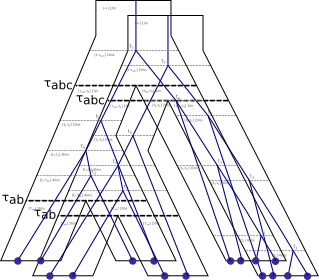
\includegraphics[width=0.6\textwidth]
{two_locus}
\caption{\textcolor{red}{A two-locus figure with migration, illustrating what statistics need to be recorded}}
\end{figure}


The summary statistics $\{numCoals(\G,p), coalStats(\G,p)\}_p$ and $\{numMigs(\G,b), migStats(\G,b)\}_b$ satisfy our first objective in that their number depends on the complexity of model the $\M$ but not on the size of the data.
%
They also partly satisfy the second condition, because statistics computed for a given set of local genealogies, $\G$, and given values of divergence times enable computation of the likelihood $P(\G|\T,\M)$ for any set of values of the population size and migration rate parameters.
%

\subsection{Sufficient Statistics Supporting Multiple Reference Models}
To support a wide variety of reference models (as stated in the second condition over sufficient stats) we must calculate $\{numCoals(\G,clade(p)), coalStats(\G,clade(p))\}_p$%
We do this by embedding the local genealogies inside $p$ into $clade(p)$ and calculating the summary statistics over the new set of intervals in the $clade(p)$. 
\begin{figure}[h]
\centering
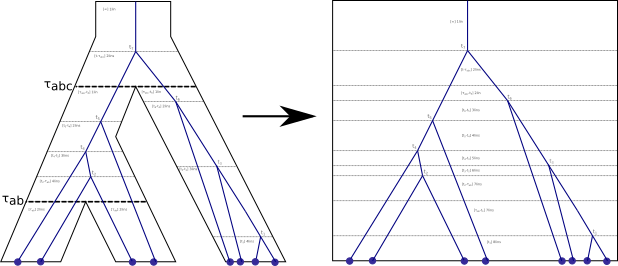
\includegraphics[width=0.8\textwidth]
{embed_in_null_model}
\caption{Embedding a local genealogy into a clade created by collapsing population $ABC$. In $clade(ABC)$, the genealogy induces a new set of intervals with different elapsed times and number of lineages. From this set we calculate $numCoals(\G,clade(ABC))$ and $coalStats(\G,clade(ABC))$ \textcolor{red}{TODO - make intervals legible}}
\end{figure}

Figure 1 illustrates embedding a single local genealogy into the null reference model. Note that the null reference model has a distinct set of intervals with different elapsed times and numbers of lineages. Computing the sufficient stats based on these intervals in population $root$  in $\Mnull$ and plugging them into formula (my7+8) would yield the value of $P(\G| \T,\Mnull)$.

To satisfy our second requirement, of supporting a wide variety of reference models, the proccess illustrated in Fig 1 must be implemented for a variety of topologies. We achieve this by clade-collapsing every subtree and caculating summary statistics over the resulting clade. This allows us to later compose a valid reference model using different pieces of topology and reuse of stats from the hypothesis model calculated by \gp.
%
To calculate summary statistics for all poossible clades in an efficient manner, calculation is done recursively down the hypothesis population tree, starting from the root. The following pseudo-python calculates $numCoals$ and $coalStats$ of a clade. It does so using a statistical utility for calculating $coalStats$ of a set of sorted intervals (\pythoninline{calculate_coal_stats}), and it accesses preexisting data from \gp (\pythoninline{num_coals_from_gphocs} \& \pythoninline{sorted_intervals_from_gphocs}):
%

\begin{python}


def recursive_num_coals(pop):
    """recursively calculate and store num of coalescence
    events in clade(pop) as well as all descendant clades"""

    pop_num_coals = num_coals_from_gphocs(pop)

    if is_leaf(pop):
        return pop_num_coals

    left_num_coals = recursive_num_coals(pop.left)
    right_num_coals = recursive_num_coals(pop.right)

    current_num_coals = pop_num_coals + left_num_coals + right_num_coals
    store(current_num_coals)

    return current_num_coals


def recursive_coal_stats(pop):
    """recursively calculate and store coalescence stats
    of clade(pop) as well as all descendant clades"""

    pop_intervals = sorted_intervals_from_gphocs(pop)

    if is_leaf(pop):
        return pop_intervals

    left_intervals = recursive_coal_stats(pop.left)
    right_intervals = recursive_coal_stats(pop.right)
    merged_intervals = merge_sort(left_intervals, right_intervals)

    clade_intervals = merged_intervals.append(pop_intervals)

    clade_coal_stats = calculate_coal_stats(clade_intervals)
    store(clade_coal_stats)

    return clade_intervals

\end{python}

\textcolor{red}{Come back to this after we explain Clade stats properly:} Calculation of summary statistics for the comb reference model is done very similiarly, but with special attention to Comb-leaves. Comb-leaves are leaf populations which are decendant to the collapsed comb population. When calculating the summary statistics of the comb itself, we only take into account intervals which occur above the comb-age (\#TODO - explain comb-age\#). Intervals below the comb-age are counted towards their original leaf population and intervals which intersect the comb-age are split into two parts - below and above the comb-age (See figure 2 for example). Using this method, full summary statistics are emitted for the comb-leaves.

\begin{figure}[h]
\centering
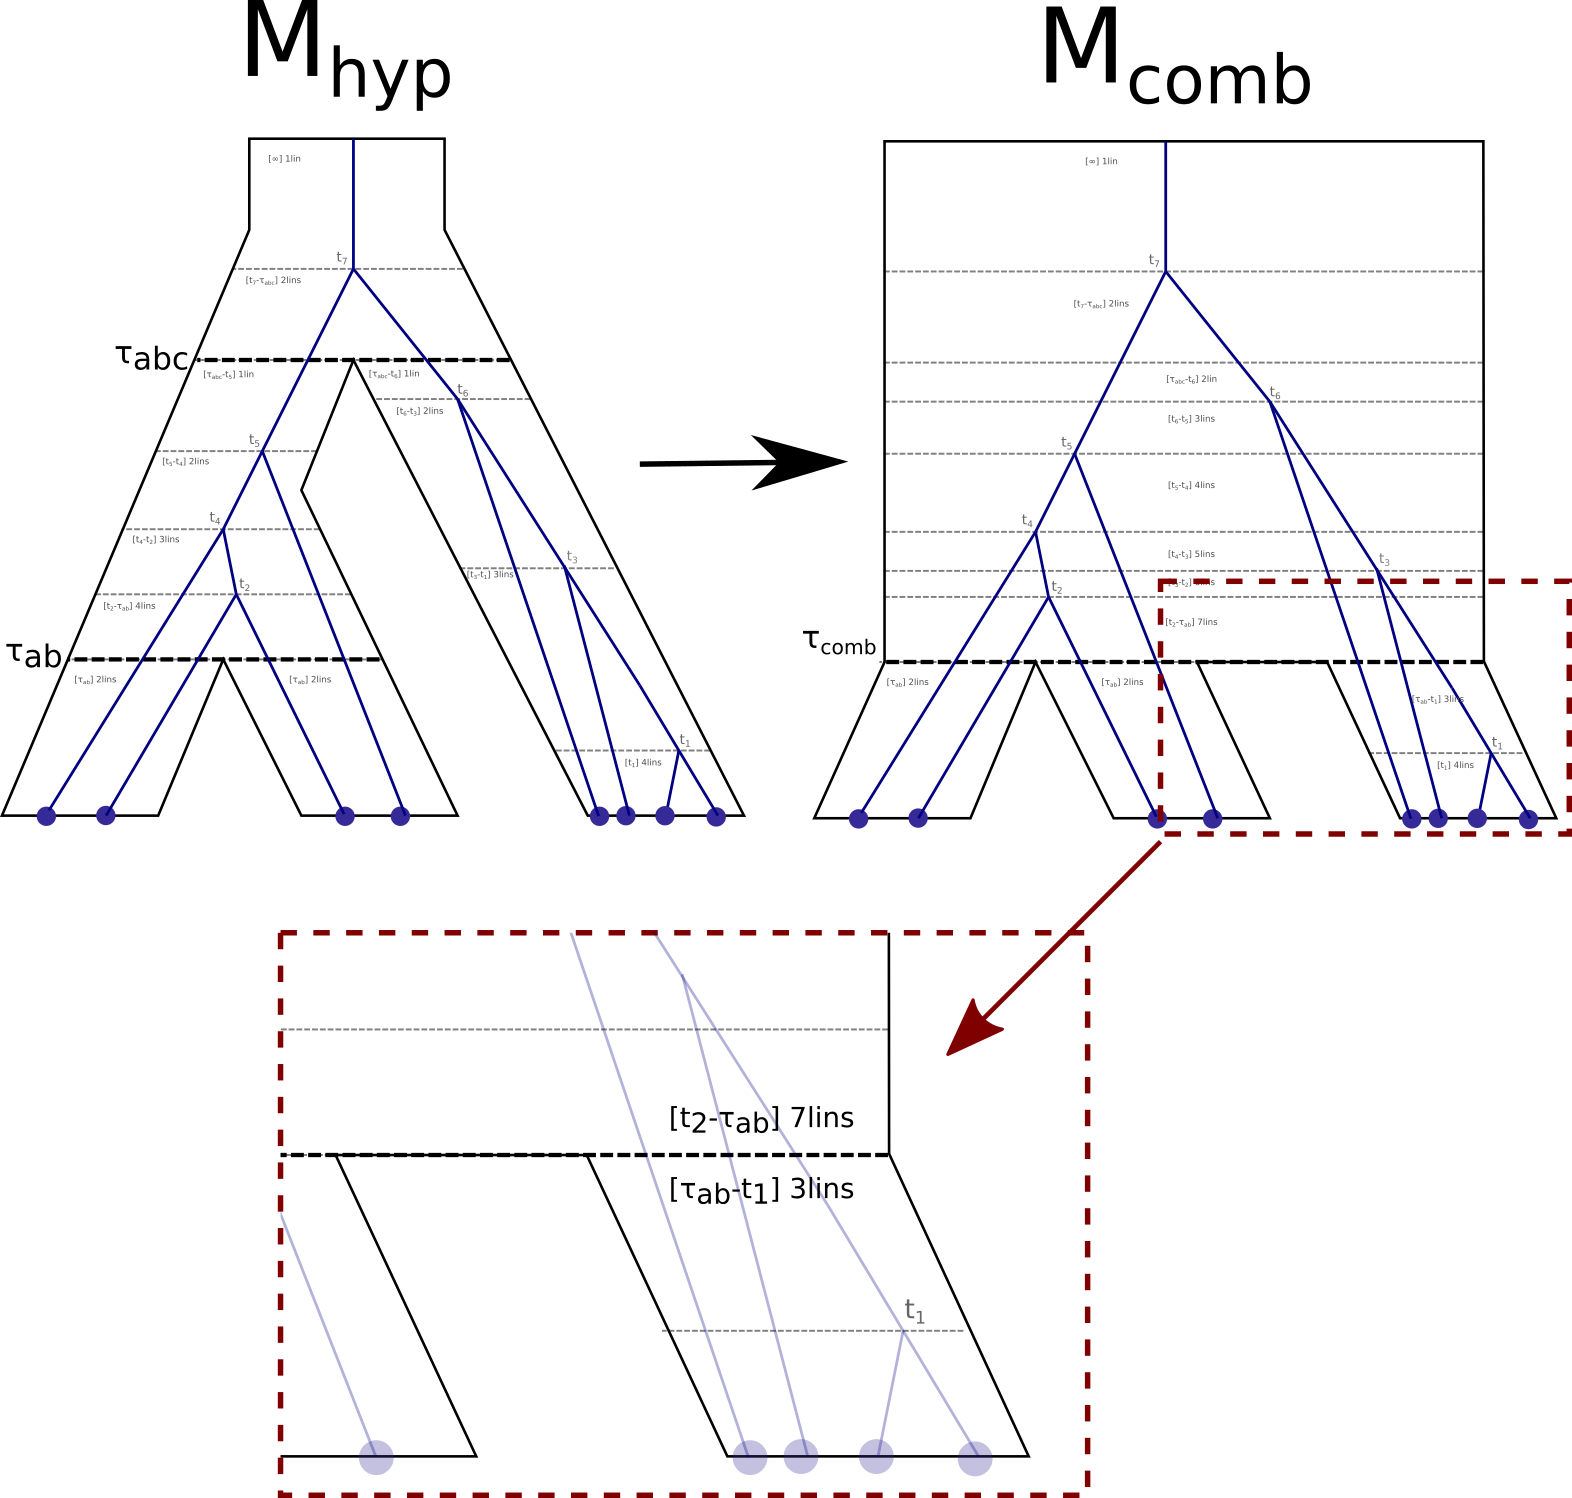
\includegraphics[width=0.8\textwidth]
{split_interval_on_comb_age}
\caption{The genealogy depicted in figure 1, embedded into a comb reference model. Intervals which span the comb-age are split to two parts - below and above the comb-age, and counted respectively toward the sufficient statistics of the comb-leaf and the comb.}
\label{fig:comb_collapse_and_split_interval}
\end{figure}

\section{Calculating sufficient statistics}


\subsection{Debugging results}

When examining results of \gp calculations for mcref we were faced with the challenge of validating our results. \#explanation-on-why-this-was-needed. We wished to double-check every statistic emitted, with the simple goal of predictably and reliably reaching our intended calculation.

This was accomplished using a variaty of techniques, restricted by the target statistic and reference model and by the tools at our disposal. 


\begin{itemize}

\item \underline{in comb: compare leaves when comb-age:=inf. Compare root comb when comb-age:=0}

To validate our comb coal-stats calculations we permanantly set the comb-age to various values, allowing us to predict results. When setting a high comb-age (essentially infinite), we asserted That the coal-stats of comb-leaves is equal to the leaf population stats calculated by \gp. When setting comb-age to zero (thus reducing the comb to a clade), we asserted that the coal-stats of the root-comb is equal those of the null reference model (calculated independently by the clade algorithm and by a preexisting \gp implementation).



\item \underline{in clade: compare "leaf clade" with leaf. Compare root-clade with \gp -calculated root-clade}
To assert clade coal-stats, we applied techniques similiar to those used for the comb algorithm. Leaf-rooted clades were compared with leaf stat calculated by \gp and the root-clade (aka the null reference modle) was compared with independantly calculated stats for the null reference model. 

\item \underline{In tau bounds: monotonouty up pop tree. Assert diff(bound, tau) neg correlated with \#loci}

We expected each tau bound to decrease towards its corresponding population tau as the number of loci increases. This due to an increase in the number of coalescence events, leading to an increase in chance of some coalescence event occurring closer to the population tau. We ran a simple set of \gp experiments using the same sequence data, changing only the number of loci in-use. We observed a negative correlation between the number of loci and the tau bound, as expected.

Another simple validation we performed was asserting that bounds are monotonously decreasing down the population tree.

\end{itemize}

\section{McRef}

\begin{itemize}
\item \underline{configuration}

When setting up mcref, several parameters are configured. The parameters pertain to standard I/O (e.g. where the trace data files are stored and where to store output), to the phylogenic population models (i.e. the structure of the reference and hypothesis models), to \gp configuration (e.g. what alpha \& beta to use for gamma priora, what print multipliers were applied to trace data when emitted by gphocs etc.), to statistical calculations (e.g. how many bootstrap iterations to run during confidence calculation and how much burn-in and sample-skip to use in genealogy likelihood calculation) and to debugging (e.g. what debug calculations to run and visualizations to emit). 

\item \underline{calculating kingman coalescence and kingman migration for the reference model}

Calculating the reference model genealogy likelihood was done using the standard kingman coalescence model, in the same manner implemented in gphocs. The theta of the actual comb/clade population was set to that of the population at the top of the comb/clade and plugged into \#gen\_ld\_ln-formula. 

\item \underline{calculating tau priors for hypothesis and reference models}
tau priors for the hypothesis model were calculated using the same gamma-distribution used by gphocs, based on taus emitted during the \gp run. tau priors for the reference model were calculated using a uniform distribution based on tau-bounds, as described in the chapter about tau bounds.

\item \underline{estimating variance using bootstrap}

In an attempt to estimate the variability of the genealogy likelihood calculation, bootstrap estimations of the rbf were repeatedly sampled from the trace data. 


\item \underline{optimizing runtime (lazily caching trace files, multiprocess concurrently running comparisons, )}

With the goal of optimizing the practical run-time and usability of mcref, several techniques were employed; trace data files, which are repeatedly read and used, are lazily loaded and cached in each mcref process. Multiple mcref experiments are launched using a single command and are cocurrently run in multiple processes, eventually aggregating summary results to a single log file. 

\item \underline{visualizing results}

To clarify results and to help in the understanding and debugging of mcref runs, several visual outputs were developed. each mcref run emits plots of the genealogy-log-likelihood of the reference model and of the hypothesis model, as well as a plot of the rbf calculation across \gp iterations and a plot of the harmonic mean of likelihood of the hypothesis model.

\item \underline{debugging visualizations}

Multiple debug plots are also emitted by mcref. Their goal is to help the researcher assert the experiment was executed as planned. These plots contain the kingman coalescence and kingman migration of every population and migration in both the hypothesis and reference models. They also contain the aggregate coal-stats of the hypothesis and reference model, allowing us to assert that coal-stats of a reference model always exceed those of it's hypothesis \#here-goes-an-explanation-of-the-previous-sentence. 
\end{itemize}



\section{Tau bounds}

\subsection{Definitions}

\subsubsection{Genealogy and Population Phylogeny}
A genealogy $G$ is a chronological binary tree whos leaves represent sampled individuals and non-leaf nodes represent coalescence events. each node $e \in G$ has an ocurrence time $t(e)$. TODO: write a more rigurous explanation of a genealogy...

A parameterized population phylogeny $P$ is a chronological binary tree whose nodes represent population-end times $\tau(p)$ (and the birth of two new populations) and whos vertices represent the time span of the population. TODO: Write a better formalization of a population phylogeny (mentioning that Leaf events are permanantly mapped to population they are "born in")...

\subsubsection{Some operators, functions and observations}

\begin{itemize}


\item $leaves(e)$ is the set of all leaf decendants of $e$

\item $father(p/e)$, $leftson(p/e)$ \& $rightson(p/e)$ are operators for traversing the population/genealogy tree

\item $mrcaPop(e)$ is the most recent population from which all populations in $\{pop(l) | l \in leaves(e)\}$ are descended


\item The binary operator $\geq^{p/e}$ between populations/events denotes the natural ancestry partial order relation between populations/events in the population/genealogy tree $P/G$. We say $p/e_1 \geq^{p/e} p/e_2$ if $p/e_1$ is ancestral or identical to $p/e_2$.
\begin{itemize}
\item Note that $p_1 \geq^p p_2 \Rightarrow \tau(p_1) \geq \tau(p_2)$
\end{itemize}

\item Note that if distict subtrees rooted at $t_1$ and $t_2$ share decendants then one must be ancestral to the another, i.e. $t_1 >_t t_2 \oplus t_2 >_t t_1 $
\end{itemize}


\subsubsection{Embeddability}


\textbf{An embedding of genealogy $G$ in phylogeny $P$} is a mapping $e \mapsto p$ denoted $pop(e)$ of all events onto populations s.t. - 

\begin{enumerate}
\item $\tau(pop(e)) < t(e) \leq \tau(father(pop(e)))$ 
\item $pop(e) \geq^p pop(leftson(e))$ and $pop(e) \geq^p pop(rightson(e))$
\end{enumerate}

Intuitively, an embedding is a population assignment to each event, that is consistent with the population phylogeny times (condition 1 ) and where each edge follows a path of ancestry (condition 2).\\

Note that if $e_1 \geq_e e_2$ then $pop(e_1) \geq_p pop(e_2)$. TODO: formally state that this is obvious.


\subsection{Uniqueness of an Embedding}
\textbf{mini Lemma:}
\begin{center}
If $G$ has an embedding in $P$ then the embedding is unique\end{center}
\textbf{Proof:} Assume to the contrary that $p_1$ \& $p_2$ are two distict populations that meet conditions 1,2,3 of embeddablity for some event $e$.

$p_1$ and $p_2$ have common decendants (as they both meet condition 2), so they must be ordered. Since they are ordered their existence cannot overlap, in contradiction to their coexistence with $e$ (as defined by conditions 1 \& 2). Hence at most one population may meet conditions 1 \& 2 of an embedding for a specific event, hence if an embedding for $G$ exists, it is unique.


\subsection{Existence of an Embedding}
\textbf{Lemma:}
\begin{center}$G \text{ has an embedding in } P \Leftrightarrow \forall e \in G, t(e) \geq \tau(mrcaPop(e))$\end{center}
\textbf{Proof:}\\

$\Rightarrow$ If $G$ has an embedding then $ \forall e \in G$, \[\forall l \in leaves(e), e \geq_e l \] \[\Downarrow\] \[\forall l \in leaves(e), pop(e) \geq_p pop(l )\] \[\Downarrow\] \[pop(e) \geq_p mrcaPop(e)\] \[\Downarrow\] \[t(e) \geq \tau(pop(e)) \geq \tau(mrcaPop(e))\]
\\
\\

$\Leftarrow$ If $ \forall e \in G, t(e) \geq \tau(mrcaPop(e))$ then :\\


Consider the set of populations ancestral to $mrcaPop(e)$. In this set there must be exactly one population coexisting with $e$; At least one since $t(e) \geq \tau(mrca_p(e))$ (and the time-span of populations is continuous from 0 to $\infty$ ) and at most one due to the same cosiderations presented in uniqueness of an embedding. Denote this population $p^*$. 	To show that that $p^* \geq_p pop(leftson(e))$ and $p^* \geq_p pop(rightson(e))$ consider w.l.o.g $pop(leftson(e))$. Since the subtrees of $p^*$ and $pop(leftson(e))$ are not disjoint (as they both contain the populations of some of $leaves(leftson(e))$), they must be ordered or identical.
Since $p^*$ coexists with $e$ and $pop(leftson(e))$ coexists with $leftson(e)$ and $t(e) > t(leaftson(e))$, population $pop(leftson(e))$ cannot be strictly ancestral to $p^*$.
Therefore $p^* \geq_p pop(leftson(e))$ and $p^* \geq_p pop(rightson(e))$, making it a proper embedding for $e$.


\subsection{Algorithm}
Given a genealogy $G$ and a Population tree $P$ without taus, we want to define the set of possible tau ranges s.t. $G$ is embeddable in $P$.\\

\begin{itemize}
\item For leaf populations - $\tau(p) = 0$ 

\item For all populations - $\tau(p) \leq \tau(father(p))$

\item For all genealogy leaves - $t(e) \geq \tau(mrcaPop(e))$

\end{itemize}
...... more explanation of the actual algorithm......\\


The following is a python snippet implementing the algorithm. The main function is \textit{find\_tau\_bounds}. For full implementation, see appendix A:



\begin{lstlisting}[language=Python]

def find_tau_bounds(root_event):
    tau_bounds = defaultdict(lambda: float('Inf'))

    _find_tau_bounds_rec(root_event, tau_bounds)

    return tau_bounds


def _find_tau_bounds_rec(event, tau_bounds):
    if event.lca_pop is not None:  # event is a leaf
        tau_bounds[event.lca_pop] = event.time
        return

    _find_tau_bounds_rec(event.left, tau_bounds)
    _find_tau_bounds_rec(event.right, tau_bounds)

    event.lca_pop = lca(event.left.lca_pop, event.right.lca_pop)

    for pop in descendants(event.lca_pop):
        tau_bounds[pop] = min(tau_bounds[pop], event.time)
\end{lstlisting}

\end{document}
